\scanpage{48}
Je veux caractériser $A$ en termes de $\widehat\Sigma^*, A^*\in\widehat\Sigma^*$ (dans le cas $A\in\Sigma$). Bien sûr, $A$ est un \deleted{\unsure{segt|segt.}} segment qui contient $A^*$, et comme $A^*\supset\partial A$, il est minimal (\deleted{\unsure{l'unique|l’un}} \unsure{qui convient|pas uniquement}) parmi les segments \inserted{de $S$} qui conti\deleted{\unsure{ent}}ennent $A^*$ -- mais cela ne suffit pas à le caractériser. Il a cependant la propriété supplémentaire,
\[
 \forall B^*\in\widehat\Sigma^*,\quad\text{on a}\quad B^*\cap A=\varnothing,\quad\text{ou }B^*\subset A
\]

\uline{NB} En fait, avec les seules conditions $\sigma1$ \unsure{à|:} $\sigma3$ sur $\Sigma$, \deleted{\unsure{c'|i}} il n'est pas vrai que la connaissance de $\widehat\Sigma^*$ redonne $\Sigma$, exemple

\figure{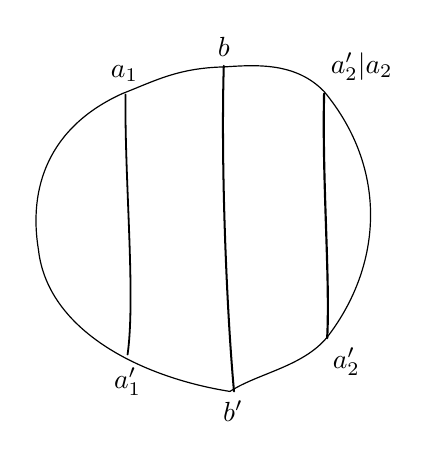
\begin{tikzpicture}[x=.013cm,y=-.013cm,line cap=round,line join=round]
\draw[line width=.43pt] (232,1287) .. controls (159,1320) and (140,1380) .. (150,1440) .. controls (159,1518) and (249,1564) .. (337,1578) .. controls (365,1560) and (408,1554) .. (432,1525) .. controls (486,1455) and (492,1361) .. (429,1285) .. controls (401,1256) and (362,1259) .. (331,1261) .. controls (286,1262) and (263,1275) .. (232,1287);
\draw[line width=.65pt] (235,1288) .. controls (234,1372) and (245,1485) .. (237,1542);
\draw[line width=.73pt] (331,1260) .. controls (328,1360) and (334,1502) .. (341,1578);
\draw[line width=.78pt] (429,1287) .. controls (427,1374) and (435,1468) .. (432,1526);
\node[above] at (234,1285) {$a_1$};
\node[above] at (331,1260) {$b$};
\node[above right] at (426,1284) {$\unsure{a'_2|a_2}$};
\node[below] at (237,1545) {$a'_1$};
\node[below] at (340,1578) {$b'$};
\node[below right] at (428,1526) {$a'_2$};
\end{tikzpicture}}
relation d'équiv. \inserted{$\unsure{\mathcal R|R}$} avec trois classes $\{a_1,a'_1\}$ $\{b,b'\}$ $\{a_2\unsure{,|{}}a'_2\}$, \inserted{\unsure{définir ici|définissons}} $\Sigma_1$ formé des segments $\{a_i,a'_i\}$ \deleted{$\unsure{\{a,a'\}|\{a_i,a'_i\}}$} $(i\in\{1,2\})$, et $\{a_1,a'_1,b,b'\}$ et $\Sigma_2$ défini de façon symétrique, définissent la $=$ $\mathcal R$\unsure{.|*}

% Four long diagonal cancellation strokes run through the following block.
\deleted{\unsure{Exemple|Énoncé} plus général: on peut de façon unique \unsure{trouver|choisir} $\Sigma$ de façon à donner}
\[
 \begin{aligned}
 &\left\{\begin{aligned}
   &\deleted{\widehat\Sigma^*=\unsure{\mathcal R|\mathcal A},\quad\text{\uuline{et}}}\\
   &\deleted{\unsure{\dot R|R}\overset{\text{déf}}{=}S\setminus\coprod_{A\in\Sigma} A=\unsure{S'|S_1|S_i},}
 \end{aligned}\right.\\
 &\qquad\deleted{\text{élément \uline{donné} d'}}\\
 &\qquad\deleted{\text{avance de }\mathcal R}\\
 &\qquad\deleted{\text{\unsure{$S'$|si} non un segment}}
 \end{aligned}
\]
% archive sheet number: 47
